\documentclass[11pt,t]{beamer}
\usepackage{graphicx}
\setbeameroption{hide notes}
\setbeamertemplate{note page}[plain]

\usetheme{default}
\beamertemplatenavigationsymbolsempty
\hypersetup{pdfpagemode=UseNone} % don't show bookmarks on initial view

% font
\usepackage{fontspec}
\setsansfont{TeX Gyre Heros}
\setbeamerfont{note page}{family*=pplx,size=\footnotesize} % Palatino for notes

\definecolor{offwhite}{RGB}{249,242,215}
\definecolor{foreground}{RGB}{255,255,255}
\definecolor{background}{RGB}{24,24,24}
\definecolor{title}{RGB}{107,174,214}
\definecolor{gray}{RGB}{155,155,155}
\definecolor{subtitle}{RGB}{102,255,204}
\definecolor{hilight}{RGB}{102,255,204}
\definecolor{vhilight}{RGB}{255,111,207}
\definecolor{lolight}{RGB}{155,155,155}

% use those colors
\setbeamercolor{titlelike}{fg=title}
\setbeamercolor{subtitle}{fg=subtitle}
\setbeamercolor{institute}{fg=gray}
\setbeamercolor{normal text}{fg=foreground,bg=background}
\setbeamercolor{item}{fg=foreground} % color of bullets
\setbeamercolor{subitem}{fg=gray}
\setbeamercolor{itemize/enumerate subbody}{fg=gray}
\setbeamertemplate{itemize subitem}{{\textendash}}
\setbeamerfont{itemize/enumerate subbody}{size=\footnotesize}
\setbeamerfont{itemize/enumerate subitem}{size=\footnotesize}

% page number
\setbeamertemplate{footline}{%
    \raisebox{5pt}{\makebox[\paperwidth]{\hfill\makebox[20pt]{\color{gray}
          \scriptsize\insertframenumber}}}\hspace*{5pt}}

% add a bit of space at the top of the notes page
\addtobeamertemplate{note page}{\setlength{\parskip}{12pt}}

% title info
\title{Avances de la tesina}
%\subtitle{A researcher's perspective}
\author{Isaí E. Dávila Cuba}
%\institute{\href{https://www.biostat.wisc.edu}{Biostatistics \& Medical Informatics} \\[2pt] \href{http://www.wisc.edu}{University of Wisconsin{\textendash}Madison}}
\date{28 de junio del 2021}

% Todos mis shorcuts para escribir más rápido.

\DeclareMathOperator{\Ran}{Ran}
\DeclareMathOperator{\Ker}{Ker}
\DeclareMathOperator{\im}{Im}



\newcommand{\imp}{\implies}			% Simbolo de implicacion
\newcommand{\supr}[1]{\underset{#1}{\sup}}
\newcommand{\mbf}[1]{\mathbf{#1}}     % Negrita en modo matemático
\newcommand{\lra}{\leftrightarrow}     % Flecha derecha e izquierda
\newcommand{\h}{\hat}             % hat para operadores
\newcommand{\red}[1]{\color{red}{#1}}
\newcommand{\green}[1]{\color{green}{#1}}
\newcommand{\blue}[1]{\color{blue}{#1}}
\newcommand{\pr}{\partial}      % Abreviacion para \partial
\newcommand{\cd}{\cdot}           % \cdot
\newcommand{\cds}{\cdots}           % \cdots
\newcommand{\inceq}{\subseteq}    % incluido e igual
\newcommand{\vc}[1]{\vec{#1}}     % vector
\newcommand{\dg}{^\dagger}
\newcommand{\conj}[1]{#1^*}       % conjugado
\newcommand{\pescalar}[2]{#1\cd #2}    % Producto escalar
\newcommand{\f}[2]{\frac{#1}{#2}}           % Short version for \frac
\newcommand{\dott}[1]{\overset{\cdot\cdot}{#1}} % Doble Punto encima (dt)
\newcommand{\nab}{\nabla}     % Shortcut for nabla
%\newcommand{\eval}{\big\rvert}  % Raya vertical para indicar evaluación
%\newcommand{\deg}[1]{#1^{\circ}}    % Grados
\newcommand{\la}{\leftarrow}        % Leftarrow
\newcommand{\mc}[1]{\mathcal{#1}}      % Tipografia caligrafia
\newcommand{\mf}[1]{\mathfrak{#1}}      % Tipografia frakture (gótico)
\newcommand{\ms}[1]{\mathscr{#1}}		% Cursiva
\newcommand{\tf}{\therefore }			% Los tres puntitos en triangulo
\newcommand{\sder}[2]{\frac{d #1}{d #2}} % Derivada simple de #1 respecto a #2
\newcommand{\der}[3]{\frac{d^{#1}#2}{d #3^{#1}}}  % Derivada n-sima de #1 respecto a #2
\newcommand{\sparc}[2]{\frac{\partial #1}{\partial #2}} %Derivadas parciales
\newcommand{\parc}[3]{\frac{\partial^{#1}#2}{\partial #3^{#1}}} %Derivada parcial n-esima respecto de #3
\newcommand{\m}[1]{\mathbb{#1}}	% Hace una letra R --> \mathbb{R}
\newcommand{\inc}{\subset}   % Incluido
\newcommand{\ndvec}[2]{(#1_1,#1_2,\ldots,#1_{#2})} %Crea un vector #2-dimensional con nombre #1
\newcommand{\ci}{\imath}		% Unidad imaginaria
\newcommand{\ptodo}{\forall}	% Para todo simbolo
\newcommand{\me}[1]{#1\m Z}		% Multiplos enteros de #1: #1Z.
\newcommand{\tq}{\mid}			% Simbolo para tal que...
\newcommand{\pp}[1]{#1^{\prime\prime}\mkern-1.2mu} %#1´´
\newcommand{\e}[1]{e^{#1}}		% Exponencial de #1
\newcommand{\om}{\omega}			% Shortcut para omega
\newcommand{\Om}{\Omega}			% Shortcut para Omega
\newcommand{\lam}{\lambda}          % Lambda
\newcommand{\Lam}{\Lambda}         % Lambda mayuscula
\newcommand{\al}{\alpha}          % alpha
\newcommand{\be}{\beta}           % beta
\newcommand{\gm}{\gamma}         % gamma
\newcommand{\Gm}{\Gamma}          % Gamma
\newcommand{\del}{\delta}         % Delta
\newcommand{\sg}{\sigma}          % Sigma
\newcommand{\Del}{\Delta}
\newcommand{\rel}{\sim}
\newcommand{\uvec}[1]{\bm{\hat{\mathbf{#1}}}}   % Vector unitario
\newcommand{\vct}[1]{\vec{\mathbf{#1}}}
\newcommand{\ra}{\rightarrow}
\newcommand{\eps}{\epsilon}
\newcommand{\ex}{\exists}
\newcommand{\bp}[1]{\left(#1\right)}
\newcommand{\bb}[1]{\left[#1\right]}
\newcommand{\bl}[1]{\left\{#1\right\}}
\newcommand{\deld}[1]{\delta^{(3)}(#1)}      % Delta de Dirac en 3d
\newcommand{\ddrc}[2]{\delta^{(#1)}(#2)}      % Delta de Dirac en Nd
\newcommand{\lrpr}{\overset{\lra}{\pr}}		% left right partial
\newcommand{\slashd}{\kern-0.5em\raise0.22ex\hbox{/}}
\newcommand{\barra}[1]{\cancel{#1}}




\usepackage[english]{babel}
\usepackage[utf8x]{inputenc}


\usepackage{amsthm, amssymb, amsfonts, amsmath}
\usepackage{graphicx}
\usepackage{tikz}
\usetikzlibrary{calc,shapes}
% \usepackage{enumitem}
\usepackage{mathtools}
\usepackage{mathrsfs}
\usepackage{tikz-cd}


\begin{document}

\begin{frame}
  \titlepage
\end{frame}

\begin{frame}{Modelo abeliano de Higgs}

$\phi:\m R^{2+1}\ra\m C$ es un campo escalar complejo acoplado al campo electromagnético mediante acoplamiento mínimo
\begin{align}
    \mc L = -\f 14 F_{\mu\nu}F^{\mu\nu}+\f 12D_\mu\phi\overline{D^\mu\phi}-\f{\lambda}8(1-|\phi|^2)^2
\end{align}
Ecuaciones de Euler-Lagrange
\begin{align}
    D_\mu D^\mu\phi+\f{\lambda}2(1-|\phi|^2)\phi &= 0\\
    \pr_\mu F^{\mu\nu} &= J^\nu
\end{align}
donde $J^\mu=\f{i}2(\bar\phi D^\mu\phi-\phi\overline{D^\mu\phi})$.
Buscamos soluciones estáticas y con energía finita. Definimos el funcional de energía $V_\lambda$
\begin{align}
    V_\lambda = \f 12\int_{\m R^2}\bp{B^2+D_i\phi\overline{D_i\phi}+\f\lambda 4(1-|\phi|^2)^2}d^2x
\end{align}

\end{frame}

\begin{frame}

Condiciones de contorno en el infinito ($|\vct x|\ra\infty$) para que $V_\lambda$ sea finita
\begin{align}
    |\phi|&\ra 1\\
    B&\ra 0\\
    D_i\phi &\ra 0
\end{align}
Estas condiciones de contorno permiten escribir el \emph{ansatz} de Nielsen-Olesen
\begin{align}
    \phi(\rho,\theta) &= f_N(\rho)e^{iN\theta}\\
    A_\theta(\rho,\theta) &= N\al_N(\rho)\\
    A_\rho &= 0
\end{align}
\begin{align}
    \f{d^2f_N}{d\rho^2}+\f{1}{\rho}\f{df_N}{d\rho}-\f{1}{\rho^2}(N-\al_N)^2 f_N+\f{\lambda}2(1-f_N^2)f_N &=0\\
    \f{d^2\al_N}{d\rho^2}-\f{1}\rho\f{d\al_N}{d\rho}+(N-\al_N)f_N^2 &= 0
\end{align}
    
\end{frame}

\begin{frame}{Soluciones numéricas}

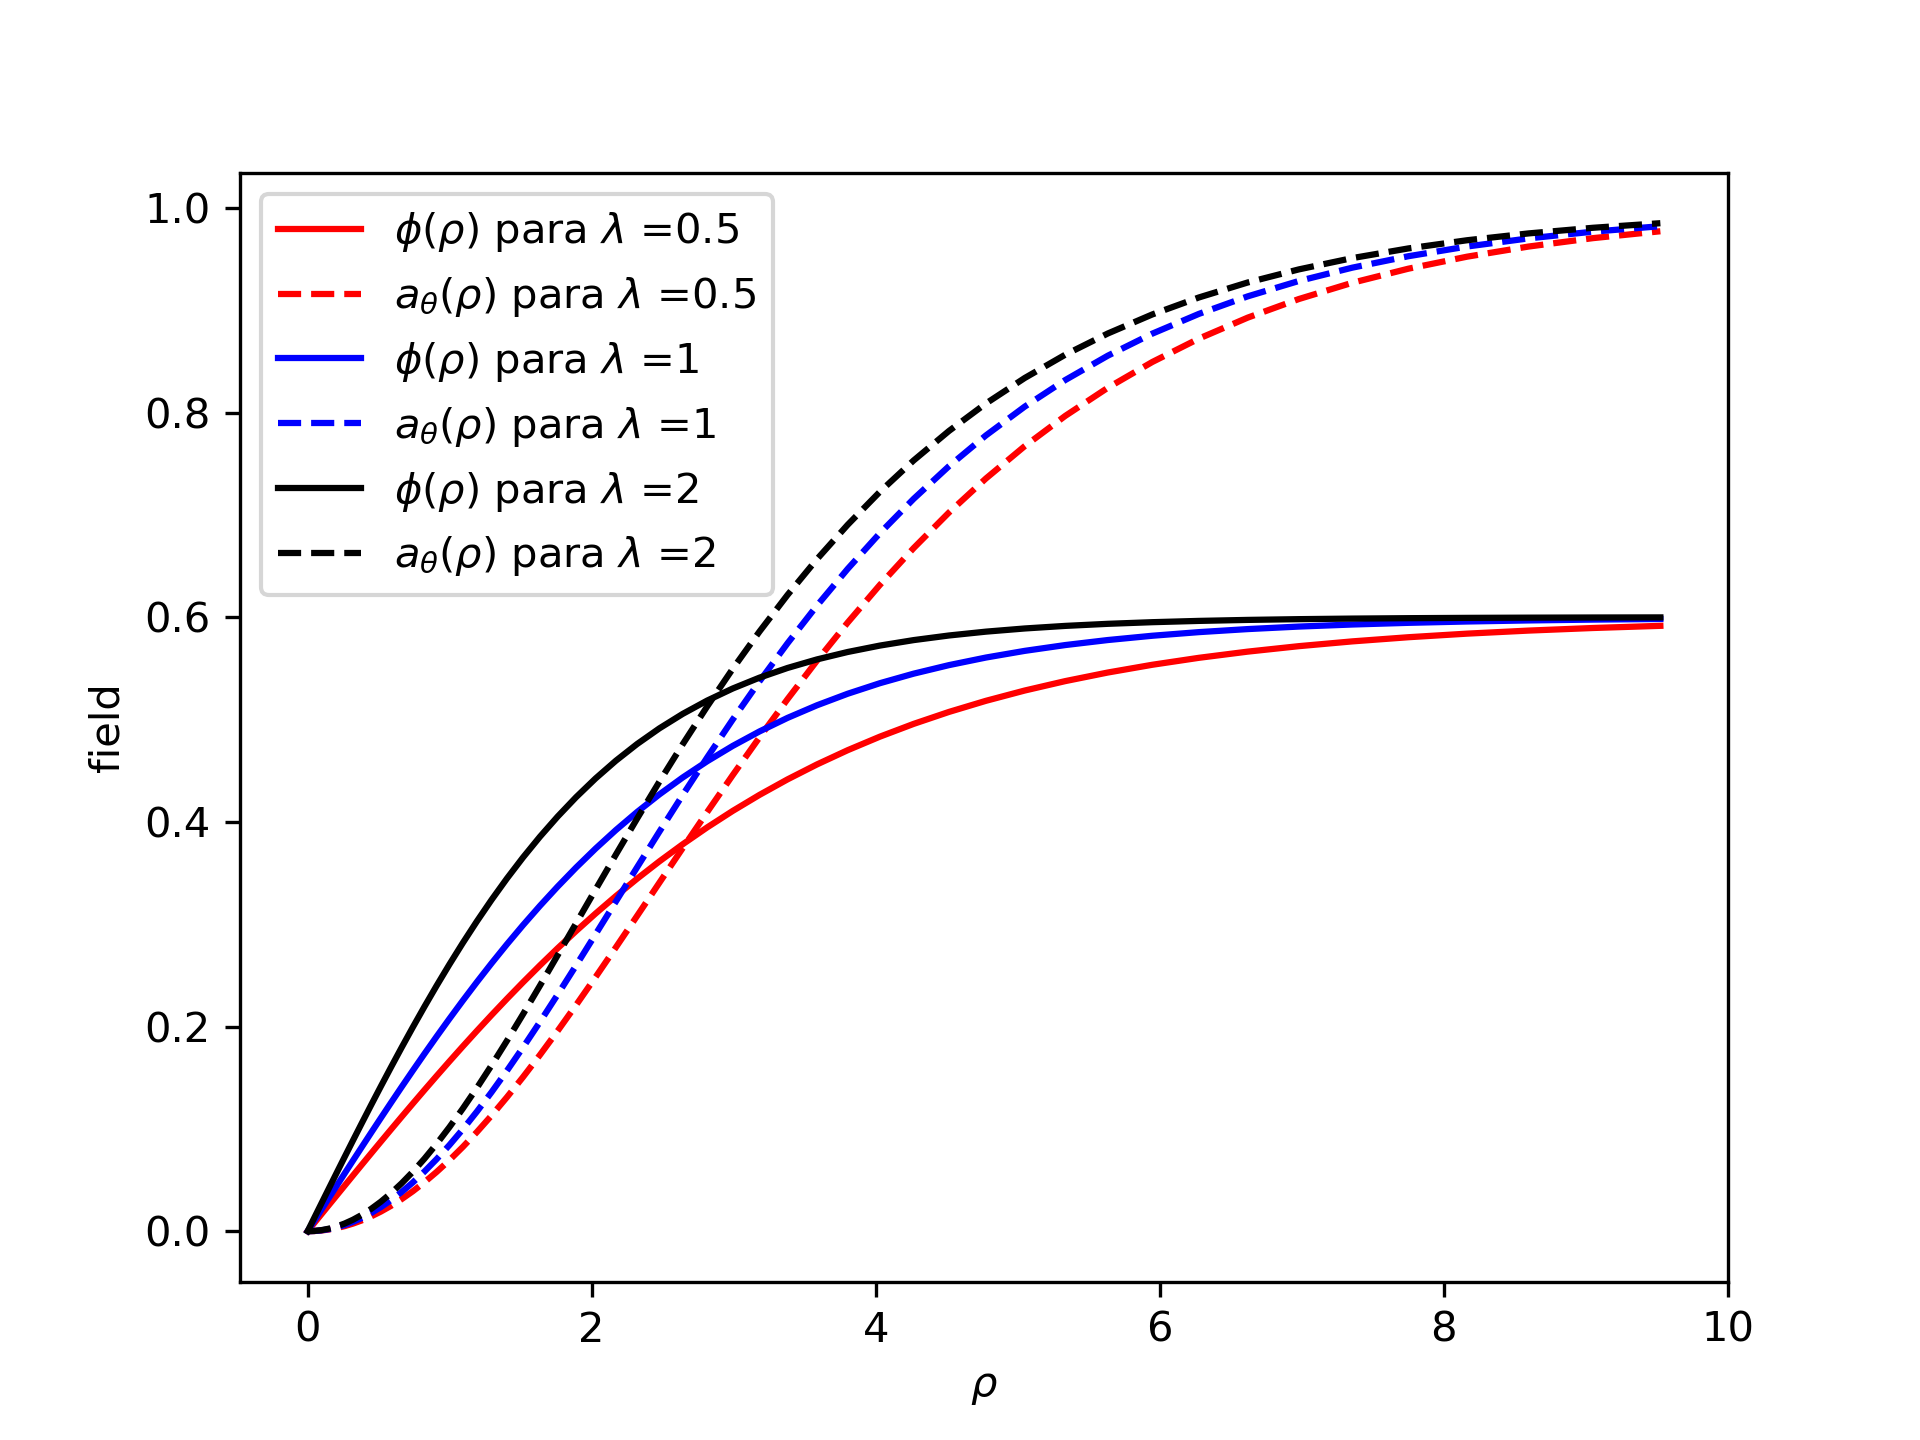
\includegraphics[width=0.5\textwidth]{fields.png}
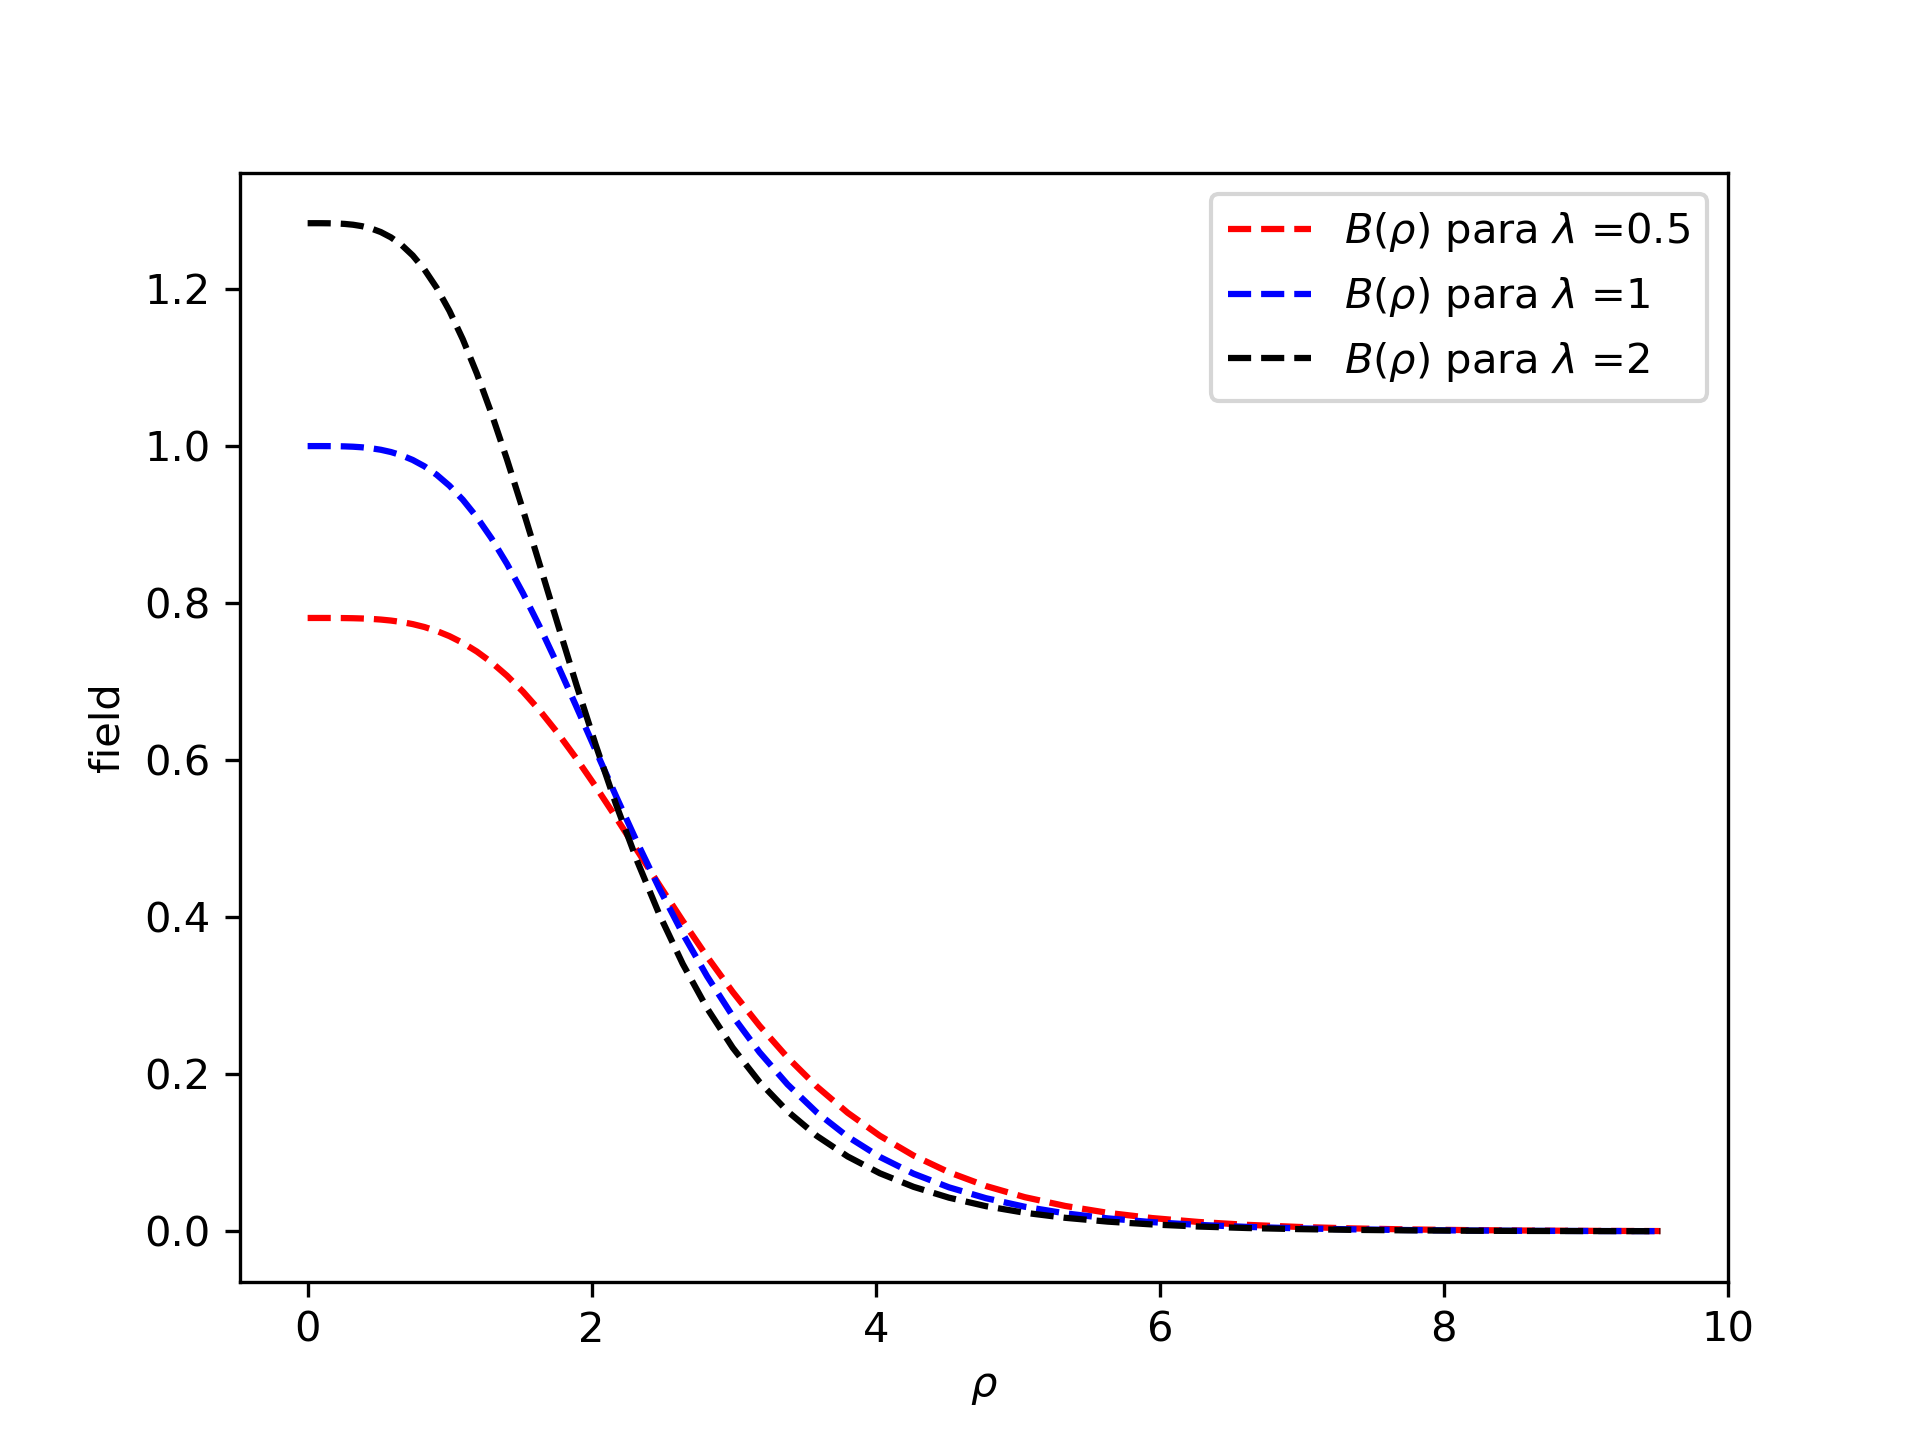
\includegraphics[width=0.5\textwidth]{Bfield.png}
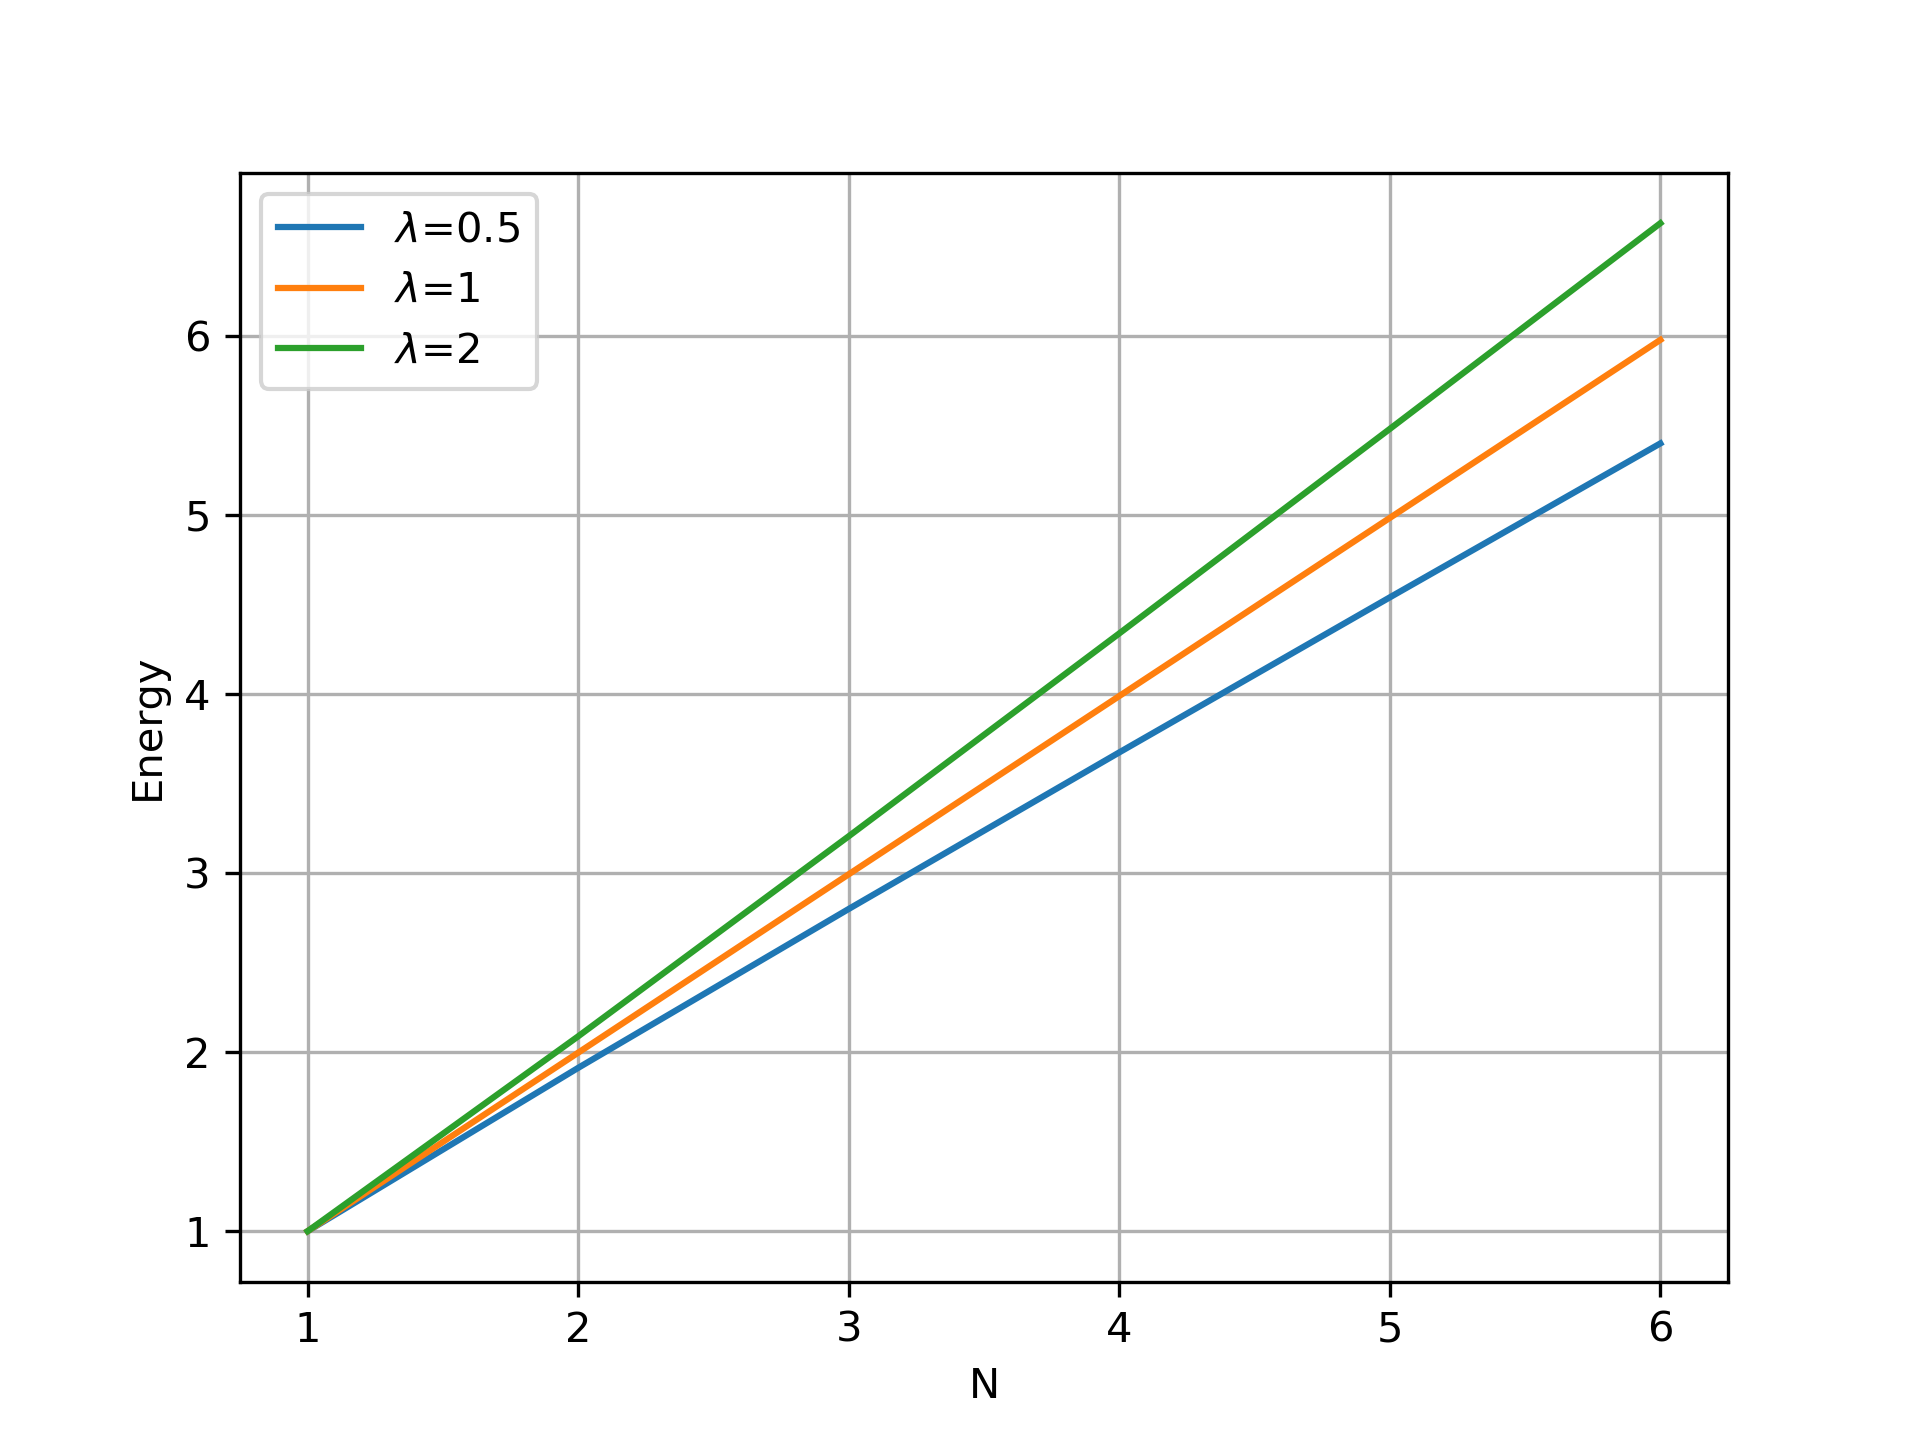
\includegraphics[width=0.5\textwidth]{Energy.png}
    
\end{frame}



% \begin{frame}
% % \frametitle{d}
%    \onslide<1->{
%    } % onslide 2
%    \onslide<1->{
%    } % onslide 3
%    \onslide<1->{
%    } % onslide 4
%    \onslide<1->{
%    } % onslide 5
%    \onslide<1->{
%    } % onslide 6
%    \onslide<1->{
%    } % onslide 7
%    \onslide<1->{
%    } % onslide 8
%    \onslide<1->{
%    } % onslide 9
%    \onslide<1->{
%    } % onslide 10
% \end{frame}


% \begin{frame}
% % \frametitle{d}
%    \onslide<1->{
%    } % onslide 2
%    \onslide<1->{
%    } % onslide 3
%    \onslide<1->{
%    } % onslide 4
%    \onslide<1->{
%    } % onslide 5
%    \onslide<1->{
%    } % onslide 6
%    \onslide<1->{
%    } % onslide 7
%    \onslide<1->{
%    } % onslide 8
%    \onslide<1->{
%    } % onslide 9
%    \onslide<1->{
%    } % onslide 10
% \end{frame}



% \begin{frame}
% % \frametitle{d}
%    \onslide<1->{
%    } % onslide 2
%    \onslide<1->{
%    } % onslide 3
%    \onslide<1->{
%    } % onslide 4
%    \onslide<1->{
%    } % onslide 5
%    \onslide<1->{
%    } % onslide 6
%    \onslide<1->{
%    } % onslide 7
%    \onslide<1->{
%    } % onslide 8
%    \onslide<1->{
%    } % onslide 9
%    \onslide<1->{
%    } % onslide 10
% \end{frame}



% \begin{frame}
% % \frametitle{d}
%    \onslide<1->{
%    } % onslide 2
%    \onslide<1->{
%    } % onslide 3
%    \onslide<1->{
%    } % onslide 4
%    \onslide<1->{
%    } % onslide 5
%    \onslide<1->{
%    } % onslide 6
%    \onslide<1->{
%    } % onslide 7
%    \onslide<1->{
%    } % onslide 8
%    \onslide<1->{
%    } % onslide 9
%    \onslide<1->{
%    } % onslide 10
% \end{frame}



% \begin{frame}
% % \frametitle{d}
%    \onslide<1->{
%    } % onslide 2
%    \onslide<1->{
%    } % onslide 3
%    \onslide<1->{
%    } % onslide 4
%    \onslide<1->{
%    } % onslide 5
%    \onslide<1->{
%    } % onslide 6
%    \onslide<1->{
%    } % onslide 7
%    \onslide<1->{
%    } % onslide 8
%    \onslide<1->{
%    } % onslide 9
%    \onslide<1->{
%    } % onslide 10
% \end{frame}


\end{document}
